\subsection{Vergelijking van de opslagsnelheden}
\label{sec:snelheden}

In tabellen \ref{tab:PL1ServeMan1}, \ref{tab:PL1ServeMan2} en \ref{tab:PL1ServeMan3} zijn de manueel gemeten opslagsnelheden weergegeven. In \ref{tab:PL1ServeAI1}, \ref{tab:PL1ServeAI2} en \ref{tab:PL1ServeAI3} zijn  de opslagsnelheden weergegeven gemaakt door Balltime AI. De eerste kolom geeft de setstanden aan. De tweede kolom geeft de speler van Lindemans Aalst aan die serveert. De derde kolom geeft de speler van Greenyard Maaseik aan die serveert en de vierde kolom geeft de snelheid in km/u aan. Op figuur \ref{fig:PL1_Serve} is een voorbeeld van de opslagmeting van Balltime AI te zien. De snelheid is weergegeven in de rechterbovenhoek van het scherm.

\begin{figure}
  \centering
  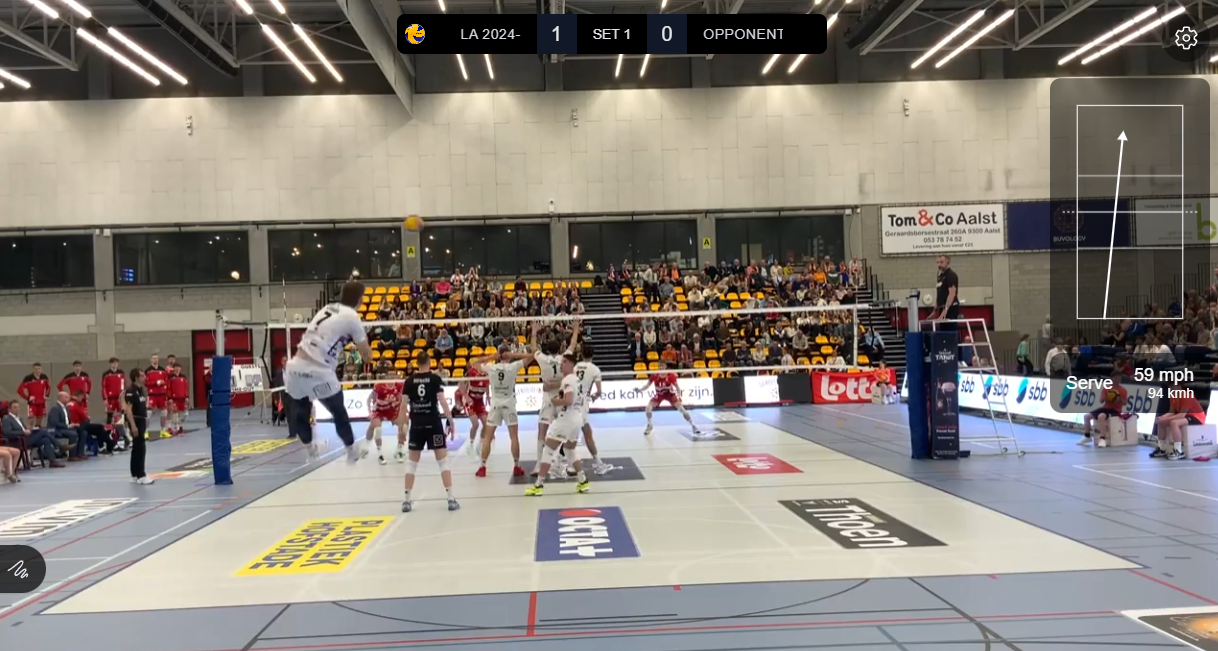
\includegraphics[width=\textwidth]{PL1_AM/opslag.png}
  \caption{\label{fig:PL1_Serve}Voorbeeld van opslagmeting van Balltime AI.}
\end{figure}

In set 1 valt op dat Balltime AI niet alle snelheden heeft opgemeten, zoals te zien is in tabel \ref{tab:PL1ServeAI1}. Er zijn maar 13 metingen gedaan terwijl er 44 opslagen zijn geweest, ongeveer een 29,55\%. Dit kan te maken hebben met het feit dat de camera niet altijd goed gericht was op de bal, waardoor de snelheid niet correct kon worden gemeten. Er zijn ook grote verschillen aanwezig in de gemeten snelheden. Een verklaring hiervoor kan zijn dat bij de manuele meting het toestel naar een geel object zoekt, idealiter de bal, maar de tribune van Lindemans Aalst is ook geel. Dit zorgt ervoor dat de snelheden soms incorrect gemeten worden. 
Balltime AI registreerde sommige snelheden aanzienlijk hoger of lager dan de manuele metingen. Bij stand 3-2 mat Balltime AI 111 km/u, terwijl de manuele meting 85 km/u aangaf. Bij 12-11 gaf de AI 109 km/u, tegenover slechts 47 km/u bij de manuele meting.

\begin{table}[ht!]
  \centering
  \scriptsize
  \begin{tabular}{|c|c|c|c|} \hline
    L.A.-G.M. & L.A. & G.M. & km/u \\ \hline
    0-0 & 7 & & 97 \\
    1-0 & 7 & & 100 \\
    2-0 & 7 & & 97 \\
    2-1 & & 14 & 43 \\
    3-1 & 1 & & 53 \\
    3-2 & & 10 & 85 \\
    4-2 & 13 & & 95 \\
    4-3 & & 15 & 79 \\
    5-3 & 9 & & 97 \\
    6-3 & 9 & & 100 \\
    6-4 & & 2 & 69 \\
    7-4 & 11 & & 101 \\
    7-5 & & 12 & 92 \\
    8-5 & 14 & & 56 \\
    8-6 & & 19 & 105 \\
    9-6 & 7 & & 63 \\
    9-7 & & 14 & 45 \\
    9-8 & & 14 & 47 \\
    10-8 & 1 & & 58 \\
    10-9 & & 10 & 103 \\
    11-9 & 13 & & 103 \\
    11-10 & & 15 & 95 \\
    11-11 & & 15 & 97 \\
    12-11 & 9 & & 47 \\
    13-11 & 9 & & 97 \\
    13-12 & & 2 & 80 \\
    14-12 & 11 & & 98 \\
    15-12 & 11 & & 56 \\
    16-12 & 11 & & 111 \\
    17-12 & 11 & & 60 \\
    17-13 & & 4 & 58 \\
    18-13 & 14 & & 76 \\
    19-13 & 14 & & 58 \\
    19-14 & & 19 & 103 \\
    19-15 & & 19 & 97 \\
    20-15 & 7 & & 98 \\
    20-16 & & 14 & 53 \\
    21-16 & 3 & & 108 \\
    21-17 & & 10 & 93 \\
    22-17 & 13 & & 100 \\
    23-17 & 13 & & 101 \\
    23-18 & & 15 & 97 \\
    24-18 & 9 & & 100 \\
    24-19 & & 2 & 101 \\
    25-19 & & & \\ \hline
  \end{tabular}
  \caption[Manueel gemeten opslagsnelheden tijdens set 1]{\label{tab:PL1ServeMan1}Manueel gemeten opslagsnelheden tijdens set 1.}
\end{table}

\begin{table}[ht!]
  \centering
  \scriptsize
  \begin{tabular}{|c|c|c|c|} \hline
    L.A.-G.M. & L.A. & G.M. & km/u \\ \hline
    0-0 & 7 & & - \\
    1-0 & 7 & & - \\
    2-0 & 7 & & - \\
    2-1 & & 14 & 48 \\
    3-1 & 1 & & - \\
    3-2 & & 10 & 111 \\
    4-2 & 13 & & 89 \\
    4-3 & & 15 & - \\
    5-3 & 9 & & - \\
    6-3 & 9 & & - \\
    6-4 & & 2 & 120 \\
    7-4 & 11 & & - \\
    7-5 & & 12 & - \\
    8-5 & 14 & & - \\
    8-6 & & 19 & - \\
    9-6 & 7 & & - \\
    9-7 & & 14 & 52 \\
    9-8 & & 14 & - \\
    10-8 & 1 & & 61 \\
    10-9 & & 10 & - \\
    11-9 & 13 & & 62 \\
    11-10 & & 15 & 122 \\
    11-11 & & 15 & 98 \\
    12-11 & 9 & & 109 \\
    13-11 & 9 & & - \\
    13-12 & & 2 & 92 \\
    14-12 & 11 & & - \\
    15-12 & 11 & & - \\
    16-12 & 11 & & - \\
    17-12 & 11 & & - \\
    17-13 & & 4 & 60 \\
    18-13 & 14 & & - \\
    19-13 & 14 & & - \\
    19-14 & & 19 & - \\
    19-15 & & 19 & - \\
    20-15 & 7 & & - \\
    20-16 & & 14 & 54 \\
    21-16 & 3 & & - \\
    21-17 & & 10 & - \\
    22-17 & 13 & & - \\
    23-17 & 13 & & - \\
    23-18 & & 15 & - \\
    24-18 & 9 & & - \\
    24-19 & & 2 & - \\
    25-19 & & & \\ \hline
  \end{tabular}
  \caption[Gemeten opslagsnelheden door Balltime AI tijdens set 1]{\label{tab:PL1ServeAI1}Gemeten opslagsnelheden door Balltime AI tijdens set 1.}
\end{table}

Ook in de tweede set, zie tabel \ref{tab:PL1ServeAI2}, valt op dat Balltime AI niet alle snelheden heeft opgemeten. In deze set zijn er 23 metingen gedaan van de 46 opslagen, 50\% van de opslagen. Dit is een verbetering ten opzichte van de eerste set, maar er zijn nog steeds veel snelheden die niet zijn gemeten. De snelheden die wel zijn gemeten, zijn ook hier weer verschillend van de manueel gemeten snelheden. Bij stand 10-9 werd manueel 80 km/u gemeten, terwijl Balltime AI 114 km/u registreerde. Een kleinere afwijking was dan wel weer te vinden bij stand 16-13, waar Balltime AI een snelheid van 41 km/u aangaf tegenover 45 km/u bij de manuele meting. Balltime AI gaf op sommige momenten wel veel hogere waardes, zoals 122 km/u bij 13-11, waar manueel slechts 55 km/u werd gemeten. In deze set lijken er ook enkele consistentere snelheden te zijn gemeten, zoals bij 1-0, waar manueel de meting 93 km/u aangaf en Balltime AI 94 km/u aangaf.

\begin{table}[ht!]
  \centering
  \scriptsize
  \begin{tabular}{|c|c|c|c|} \hline
    L.A.-G.M. & L.A. & G.M. & km/u \\ \hline
    0-0 &  & 19 & 116 \\
    1-0 & 7 & & 93 \\
    1-1 &  & 14 & 50 \\
    2-1 & 1 & & 51 \\
    3-1 & 1 & & 53 \\
    3-2 &  & 10 & 95 \\
    4-2 & 13 & & 89 \\
    4-3 &  & 15 & 71 \\
    5-3 & 9 & & 97 \\
    5-4 &  & 2 & 90 \\
    6-4 & 11 & & 82 \\
    6-5 &  & 4 & 61 \\
    7-5 & 14 & & 53 \\
    7-6 &  & 19 & 116 \\
    8-6 & 7 &  & 101 \\
    8-7 &  & 14 & 55 \\
    8-8 &  & 14 & 58 \\
    9-8 & 7 & & 60 \\
    9-9 &  & 10 & 106 \\
    10-9 & 13 & & 80 \\
    11-9 & 13 & & 95 \\
    12-9 & 13 & & 97 \\
    12-10 &  & 15 & 109 \\
    12-11 &  & 15 & 92 \\
    13-11 & 9 &  & 55 \\
    13-12 &  & 2 & 93 \\
    14-12 & 11 &  & 98 \\
    14-13 &  & 4 & 53 \\
    15-13 & 14 &  & 51 \\
    16-13 & 14 &  & 45 \\
    16-14 &  & 19 & 114 \\
    17-14 & 7 &  & 105 \\
    18-14 & 7 &  & 100 \\
    18-15 &  & 14 & 50 \\
    18-16 &  & 14 & 58 \\
    19-16 & 3 &  & 106 \\
    20-16 & 3 &  & 98 \\
    20-17 &  & 10 & 105 \\
    21-17 & 13 &  & 97 \\
    22-17 & 13 &  & 106 \\
    23-17 & 13 &  & 100 \\
    23-18 &  & 15 & 58 \\
    23-19 &  & 15 & 79 \\
    24-19 & 9 &  & 98 \\
    24-20 &  & 2 & 108 \\
    24-21 &  & 2 & 101 \\
    25-21 &  &  &  \\ \hline
  \end{tabular}
  \caption[Manueel gemeten opslagsnelheden tijdens set 2]{\label{tab:PL1ServeMan2}Manueel gemeten opslagsnelheden tijdens set 2.}
\end{table}

\begin{table}[ht!]
  \centering
  \scriptsize
  \begin{tabular}{|c|c|c|c|} \hline
    L.A.-G.M. & L.A. & G.M. & km/u \\ \hline
    0-0 &  & 19 & - \\
    1-0 & 7 & & 94 \\
    1-1 &  & 14 & 56 \\
    2-1 & 1 & & 55 \\
    3-1 & 1 & & 59 \\
    3-2 &  & 10 & - \\
    4-2 & 13 & & - \\
    4-3 &  & 15 & - \\
    5-3 & 9 & & - \\
    5-4 &  & 2 & 95 \\
    6-4 & 11 & & - \\
    6-5 &  & 4 & - \\
    7-5 & 14 & & 71 \\
    7-6 &  & 19 & - \\
    8-6 & 7 &  & 70 \\
    8-7 &  & 14 & 54 \\
    8-8 &  & 14 & 43 \\
    9-8 & 7 & & 73 \\
    9-9 &  & 10 & 92 \\
    10-9 & 13 & & 114 \\
    11-9 & 13 & & 109 \\
    12-9 & 13 & & 98 \\
    12-10 &  & 15 & - \\
    12-11 &  & 15 & 74 \\
    13-11 & 9 &  & 122 \\
    13-12 &  & 2 & - \\
    14-12 & 11 &  & - \\
    14-13 &  & 4 & 52 \\
    15-13 & 14 &  & 113 \\
    16-13 & 14 &  & 41 \\
    16-14 &  & 19 & - \\
    17-14 & 7 &  & - \\
    18-14 & 7 &  & 53 \\
    18-15 &  & 14 & 49 \\
    18-16 &  & 14 & - \\
    19-16 & 3 &  & - \\
    20-16 & 3 &  & - \\
    20-17 &  & 10 & - \\
    21-17 & 13 &  & 118 \\
    22-17 & 13 &  & - \\
    23-17 & 13 &  & - \\
    23-18 &  & 15 & - \\
    23-19 &  & 15 & - \\
    24-19 & 9 &  & 33 \\
    24-20 &  & 2 & - \\
    24-21 &  & 2 & - \\
    25-21 &  &  &  \\ \hline
  \end{tabular}
  \caption[Gemeten opslagsnelheden door Balltime AI tijdens set 2]{\label{tab:PL1ServeAI2}Gemeten opslagsnelheden door Balltime AI tijdens set 2.}
\end{table}

Tijdens de laatste set zijn er het minste aantal metingen gedaan door Balltime AI, zie tabel \ref{tab:PL1ServeAI3}. In deze set zijn er maar 10 metingen gedaan van de 43 opslagen, slechts 23,3\%. Dit is een grote daling ten opzichte van de vorige sets. De snelheden die wel zijn gemeten liggen wel dichter bij de manuele metingen, buiten enkele uitschieters. Een verschil van 40 km/u bij stand 15-11 tussen de manuele metingen van 106 km/u en de AI meting van 66 km/u is wel opmerkelijk. Ook bij stand 24-17 is er een groot verschil. Balltime AI gaf hier een snelheid aan van 125 km/u, terwijl de manuele meting slechts 103 km/u aangaf.

\begin{table}[ht!]
  \centering
  \scriptsize
  \begin{tabular}{|c|c|c|c|} \hline
    L.A.-G.M. & L.A. & G.M. & km/u \\ \hline
    0-0 & 7 & & 61 \\
    1-0 & 7 & & 89 \\
    2-0 & 7 & & 103 \\
    3-0 & 7 & & 105 \\
    4-0 & 7 & & 108 \\
    5-0 & 7 & & 98 \\
    5-1 & & 14 & 56 \\
    5-2 & & 14 & 53 \\
    6-2 & 1 & & 58 \\
    6-3 & & 10 & 60 \\
    6-4 & & 10 & 103 \\
    7-4 & 13 & & 93 \\
    7-5 &  & 13 & 56 \\
    8-5 & 9 & & 92 \\
    8-6 &  & 2 & 97 \\
    9-6 & 11 & & 60 \\
    10-6 & 11 & & 105 \\
    11-6 & 11 & & 101 \\
    11-7 & & 12 & 84 \\
    12-7 & 14 & & 55 \\
    13-7 & 14 & & 50 \\
    13-8 & & 19 & 100 \\
    13-9 & & 19 & 100 \\
    14-9 & 7 & & 103 \\
    14-10 & & 14 & 56 \\
    15-10 & 1 & & 60 \\
    15-11 & & 10 & 106 \\
    16-11 & 13 & & 98 \\
    17-11 & 13 & & 114 \\
    18-11 & 13 & & 111 \\
    19-11 & 13 & & 113 \\
    20-11 & 13 & & 69 \\
    21-11 & 13 & & 92 \\
    21-12 & & 15 & 76 \\
    21-13 & & 15 & 69 \\
    22-13 & 9 & & 97 \\
    22-14 & & 2 & 69 \\
    22-15 & & 2 & 71 \\
    23-15 & 11 & & 68 \\
    23-16 & & 12 & 84 \\
    24-16 & 14 & & 53 \\
    24-17 & & 19 & 103 \\
    24-18 & & 19 & 101 \\
    25-18 & & & \\ \hline
  \end{tabular}
  \caption[Manueel gemeten opslagsnelheden tijdens set 3]{\label{tab:PL1ServeMan3}Manueel gemeten opslagsnelheden tijdens set 3.}
\end{table}

\begin{table}[ht!]
  \centering
  \scriptsize
  \begin{tabular}{|c|c|c|c|} \hline
    L.A.-G.M. & L.A. & G.M. & km/u \\ \hline
    0-0 & 7 & & - \\
    1-0 & 7 & & - \\
    2-0 & 7 & & - \\
    3-0 & 7 & & - \\
    4-0 & 7 & & - \\
    5-0 & 7 & & - \\
    5-1 & & 14 & 44 \\
    5-2 & & 14 & 44 \\
    6-2 & 1 & & 52 \\
    6-3 & & 10 & - \\
    6-4 & & 10 & - \\
    7-4 & 13 & & - \\
    7-5 &  & 13 & - \\
    8-5 & 9 & & - \\
    8-6 &  & 2 & - \\
    9-6 & 11 & & - \\
    10-6 & 11 & & - \\
    11-6 & 11 & & - \\
    11-7 & & 12 & - \\
    12-7 & 14 & & - \\
    13-7 & 14 & & - \\
    13-8 & & 19 & - \\
    13-9 & & 19 & - \\
    14-9 & 7 & & - \\
    14-10 & & 14 & 50 \\
    15-10 & 1 & & 59 \\
    15-11 & & 10 & 66 \\
    16-11 & 13 & & - \\
    17-11 & 13 & & - \\
    18-11 & 13 & & - \\
    19-11 & 13 & & - \\
    20-11 & 13 & & - \\
    21-11 & 13 & & - \\
    21-12 & & 15 & - \\
    21-13 & & 15 & - \\
    22-13 & 9 & & 113 \\
    22-14 & & 2 & 78 \\
    22-15 & & 2 & - \\
    23-15 & 11 & & - \\
    23-16 & & 12 & - \\
    24-16 & 14 & & - \\
    24-17 & & 19 & 125 \\
    24-18 & & 19 & 105 \\
    25-18 & & & \\ \hline
  \end{tabular}
  \caption[Gemeten opslagsnelheden door Balltime AI tijdens set 3]{\label{tab:PL1ServeAI3}Gemeten opslagsnelheden door Balltime AI tijdens set 3.}
\end{table}